\chapter{Test and Results}
\label{ch:test-results}

This chapter reports the empirical evaluation of the three offline models
introduced in Chapter~\ref{ch:implementation} together with the on-device
behavior of the Android demonstration application. The aim is twofold.
First, to verify that each model meets the acceptance criteria specified
in the project proposal: a Top-1 accuracy of at least 40\,\% on the
WLASL-100 word-recognition task and a confident letter classifier for
the ASL Alphabet. Second, to make the deployability claim of this
thesis quantitative by comparing the four classifiers along axes that
matter on a phone: accuracy, model size and inference latency.

%==============================================================================
\section{Evaluation Methodology}
\label{sec:results-methodology}

All offline results in this chapter are computed on the held-out test
splits described in Section~\ref{sec:impl-data}. The ASL Alphabet
classifiers are evaluated on the 13\,050-image test partition produced
by the 70/15/15 stratified split; the word classifiers are evaluated on
the 201-clip test partition that follows the official WLASL-100 split.
No checkpoint selection, hyperparameter tuning or threshold calibration
was performed on the test partition: the test set was held out until
the validation-best checkpoints had been frozen.

For each classification task the following metrics are reported.
\textbf{Top-1 accuracy} is the share of samples whose argmax prediction
matches the ground truth. \textbf{Top-5 accuracy} is the share of
samples whose ground-truth label appears in the five highest-scoring
predictions; it is informative for the word task, where confusable
near-synonyms make Top-1 the harder metric. \textbf{Macro F1} averages
the per-class F1 score with equal weight, which makes it sensitive to
the under-represented classes that the
\texttt{WeightedRandomSampler} of Section~\ref{sec:impl-lstm-training}
was designed to support. \textbf{Weighted F1} weighs each class by its
support and is reported alongside Macro~F1 for completeness. Confusion
matrices are visualized to expose systematic error patterns.

For deployment metrics, \textbf{model size} is the on-disk size of the
serialized checkpoint (PyTorch \texttt{state\_dict} for the offline
numbers, TensorFlow~Lite flatbuffer for the on-device numbers).
\textbf{Inference latency} is measured as the mean time spent inside
the classifier's \texttt{forward} pass on a single sample, with a 50-batch
warm-up and a 200-sample timed window. \textbf{Frames per second} is
the reciprocal of the latency. Two latency budgets are reported per
model: an offline budget measured on the training GPU, and an
on-device budget measured on the Android test phone
(Chapter~\ref{ch:implementation}); the latter is the deployment-relevant
number.

The word classifier is trained five times with different random seeds,
and the per-seed accuracies are reported individually alongside the
five-seed ensemble. The image and MLP letter classifiers are trained
once with a fixed seed; their accuracy ceiling is high enough that
seed-to-seed variance does not change the conclusions, and the focus of
the letter comparison is the architectural trade-off between an image
network and a landmark network rather than the variance of either one.

Three caveats apply throughout the chapter and are stated here once.
First, the ASL Alphabet split is random rather than person-disjoint,
because the public dataset does not expose signer identity. This is a
known limitation of single-source datasets and means that the
100\,\% and 99.38\,\% letter accuracies should be interpreted as
in-distribution upper bounds rather than as predictions of real-world
generalization. Real-device behavior on previously unseen hands is
revisited in Section~\ref{sec:results-on-device}. Second, the WLASL-100
split is person-mixed by design: the same signer can appear in both
train and test partitions, which inflates the absolute Top-1 number
relative to a strict signer-disjoint protocol. Third, the word
classifier's test partition contains only 201 clips and two classes
have zero test examples (\texttt{later} and \texttt{book}), so
single-class metrics on those classes are undefined and the macro
F1 averages over 98 effective classes.

%==============================================================================
\section{Letter Recognition Results}
\label{sec:results-letters}

Both letter classifiers reach near-ceiling accuracy on the ASL Alphabet
test partition. EfficientNet-B0 produces \emph{zero} misclassifications
on the 13\,050 test images and therefore reaches a Top-1 accuracy of
exactly 100\,\%, with a per-class F1 score of 1.000 across all
29 classes. The landmark MLP reaches 99.38\,\% Top-1 accuracy on the
subset of test images for which MediaPipe successfully detected a hand
(73.09\,\% of the test partition, as discussed in
Section~\ref{sec:impl-mlp}). The two numbers therefore measure two
different effective populations: the image classifier evaluates on the
complete test set, while the landmark classifier evaluates on the
detector-recoverable subset and is undefined on the remaining
\SI{26.91}{\percent} of images.

\begin{table}[h]
\centering
\caption{Test-set accuracy and footprint of the two letter classifiers.}
\label{tab:results-letters}
\begin{tabular}{lcc}
\toprule
\textbf{Metric} & \textbf{EfficientNet-B0} & \textbf{Landmark MLP} \\
\midrule
Top-1 accuracy           & 100.00\,\%         & 99.38\,\% \\
Per-class F1 (mean)      & 1.000               & 0.994 \\
Coverage on test split   & 100.00\,\%         & 73.09\,\% \\
Parameters               & 4.1\,M              & 60\,K \\
Checkpoint size          & 15.71\,MB          & 0.24\,MB \\
Offline latency (GPU)    & 2.04\,ms / sample  & 0.01\,ms / sample \\
Offline throughput (GPU) & 490\,FPS            & \num{91650}\,FPS \\
External dependencies    & None                & MediaPipe Hands \\
\bottomrule
\end{tabular}
\end{table}

The confusion matrices of the two letter classifiers are reported
in Figure~\ref{fig:results-cm-cnn} and
Figure~\ref{fig:results-cm-mlp}. The EfficientNet-B0 matrix is
exactly diagonal: the network produces zero off-diagonal predictions
across all 29 classes of the test partition. The landmark MLP matrix
is dominated by the same diagonal but exhibits a small number of
off-diagonal cells in the low single digits, concentrated around the
classes whose handshape MediaPipe captures less reliably
(\textit{M}/\textit{N}, \textit{R}/\textit{U}/\textit{V}). No pair of
classes is systematically confused: the largest single off-diagonal
cell remains below \SI{2}{\percent}, which is consistent with the
near-ceiling 99.38\,\% Top-1 reported in
Table~\ref{tab:results-letters}.

\begin{figure}[h]
\centering
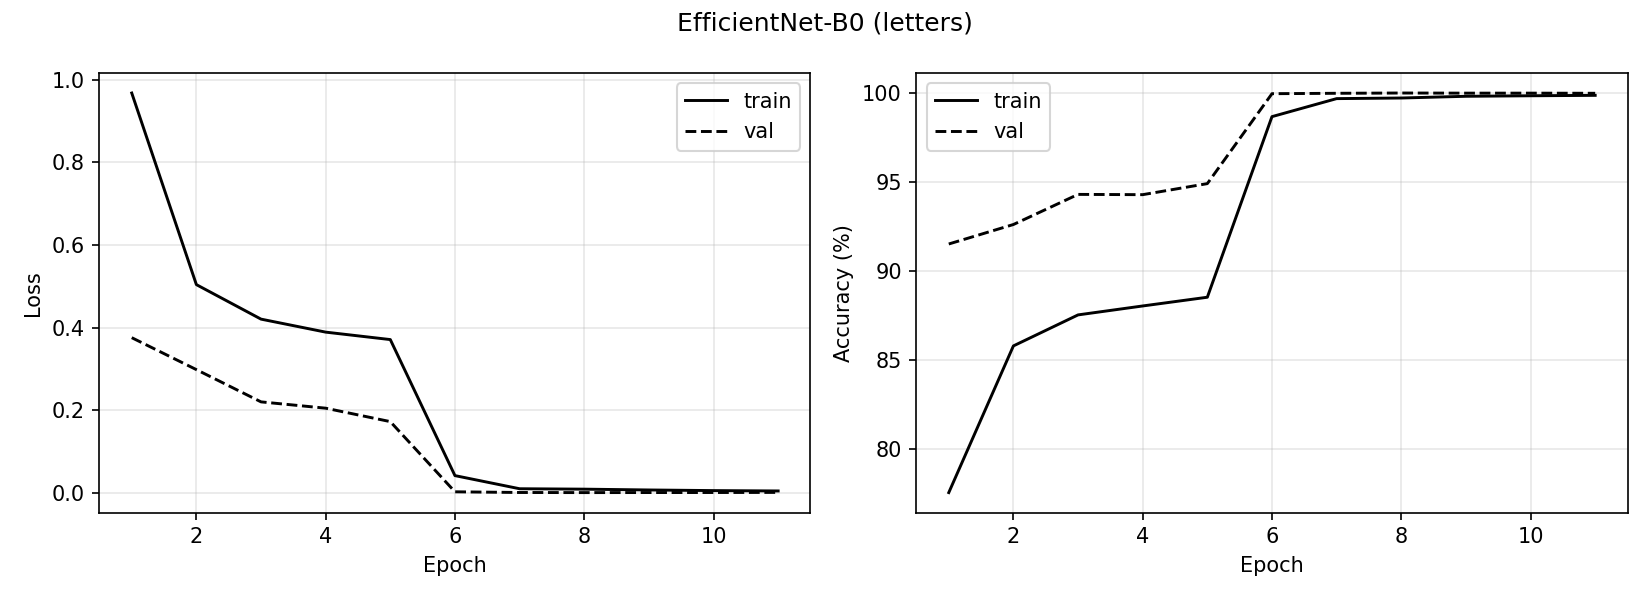
\includegraphics[width=\textwidth]{figures/ch5_lc_cnn.png}
\caption{Training trajectory of the EfficientNet-B0 letter
classifier. Both train and validation loss collapse within the
first six epochs and validation accuracy saturates at
\SI{100}{\percent} from epoch~7 onward, which triggered the
early-stopping criterion at epoch~11. The narrow train--val gap
indicates that no overfitting developed despite the large
\num{60900}-image training partition.}
\label{fig:results-lc-cnn}
\end{figure}

\begin{figure}[h]
\centering
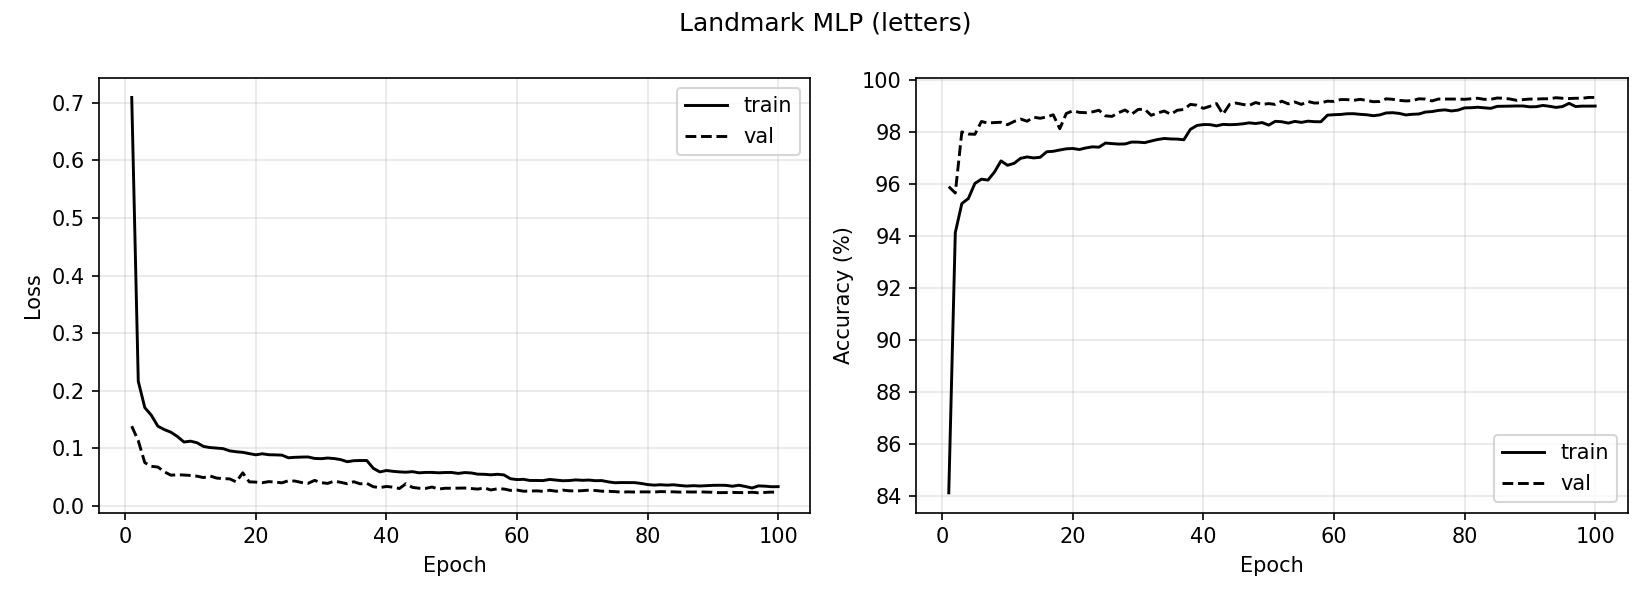
\includegraphics[width=\textwidth]{figures/ch5_lc_mlp.png}
\caption{Training trajectory of the landmark MLP letter
classifier. Validation accuracy crosses \SI{98}{\percent} within
the first ten epochs and plateaus near \SI{99.3}{\percent} for the
remaining \num{90} epochs. The validation curve remains
consistently above the training curve throughout, which is the
expected pattern when dropout regularisation is active during
training but disabled at inference.}
\label{fig:results-lc-mlp}
\end{figure}

\begin{figure}[h]
\centering
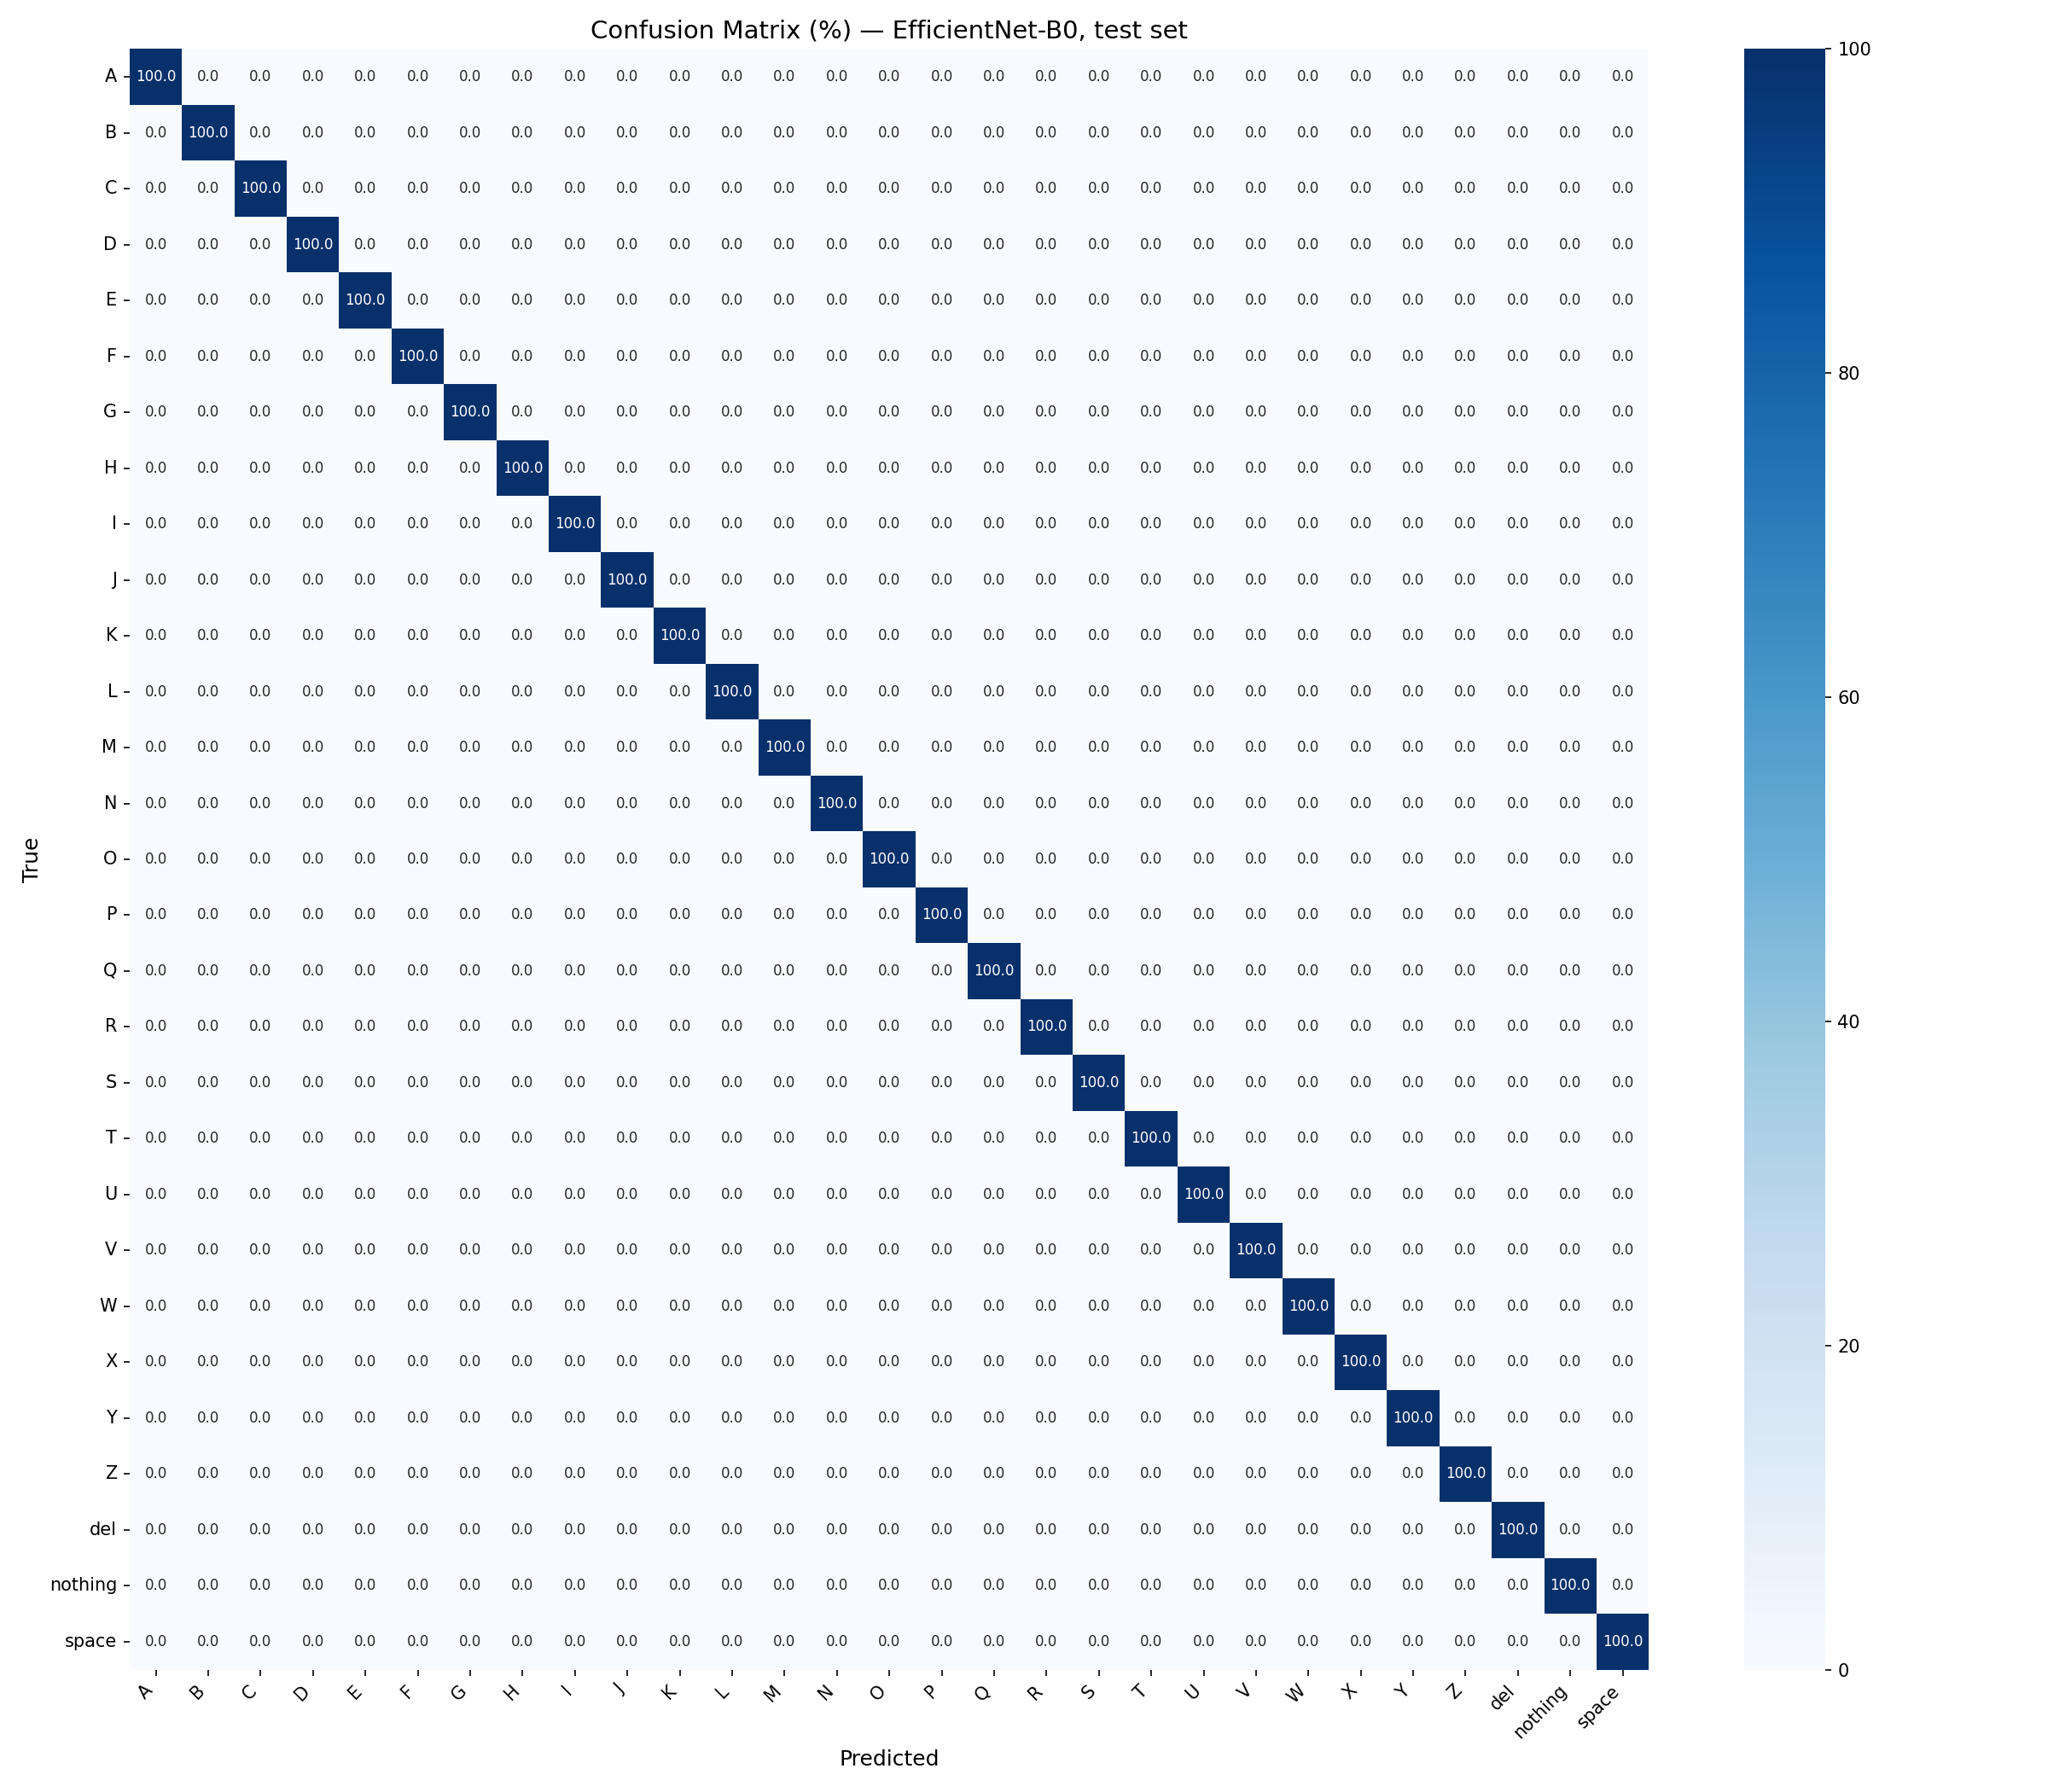
\includegraphics[width=0.9\textwidth]{figures/ch5_cm_cnn_letters.png}
\caption{Row-normalised confusion matrix of the EfficientNet-B0
letter classifier on the 13\,050-image ASL Alphabet test partition.
Cells report the percentage of true class~$y$ predicted as
class~$\hat{y}$. The matrix is strictly diagonal: the network
produces zero off-diagonal predictions across all 29 classes,
matching the 100\,\% Top-1 accuracy of
Table~\ref{tab:results-letters}.}
\label{fig:results-cm-cnn}
\end{figure}

\begin{figure}[h]
\centering
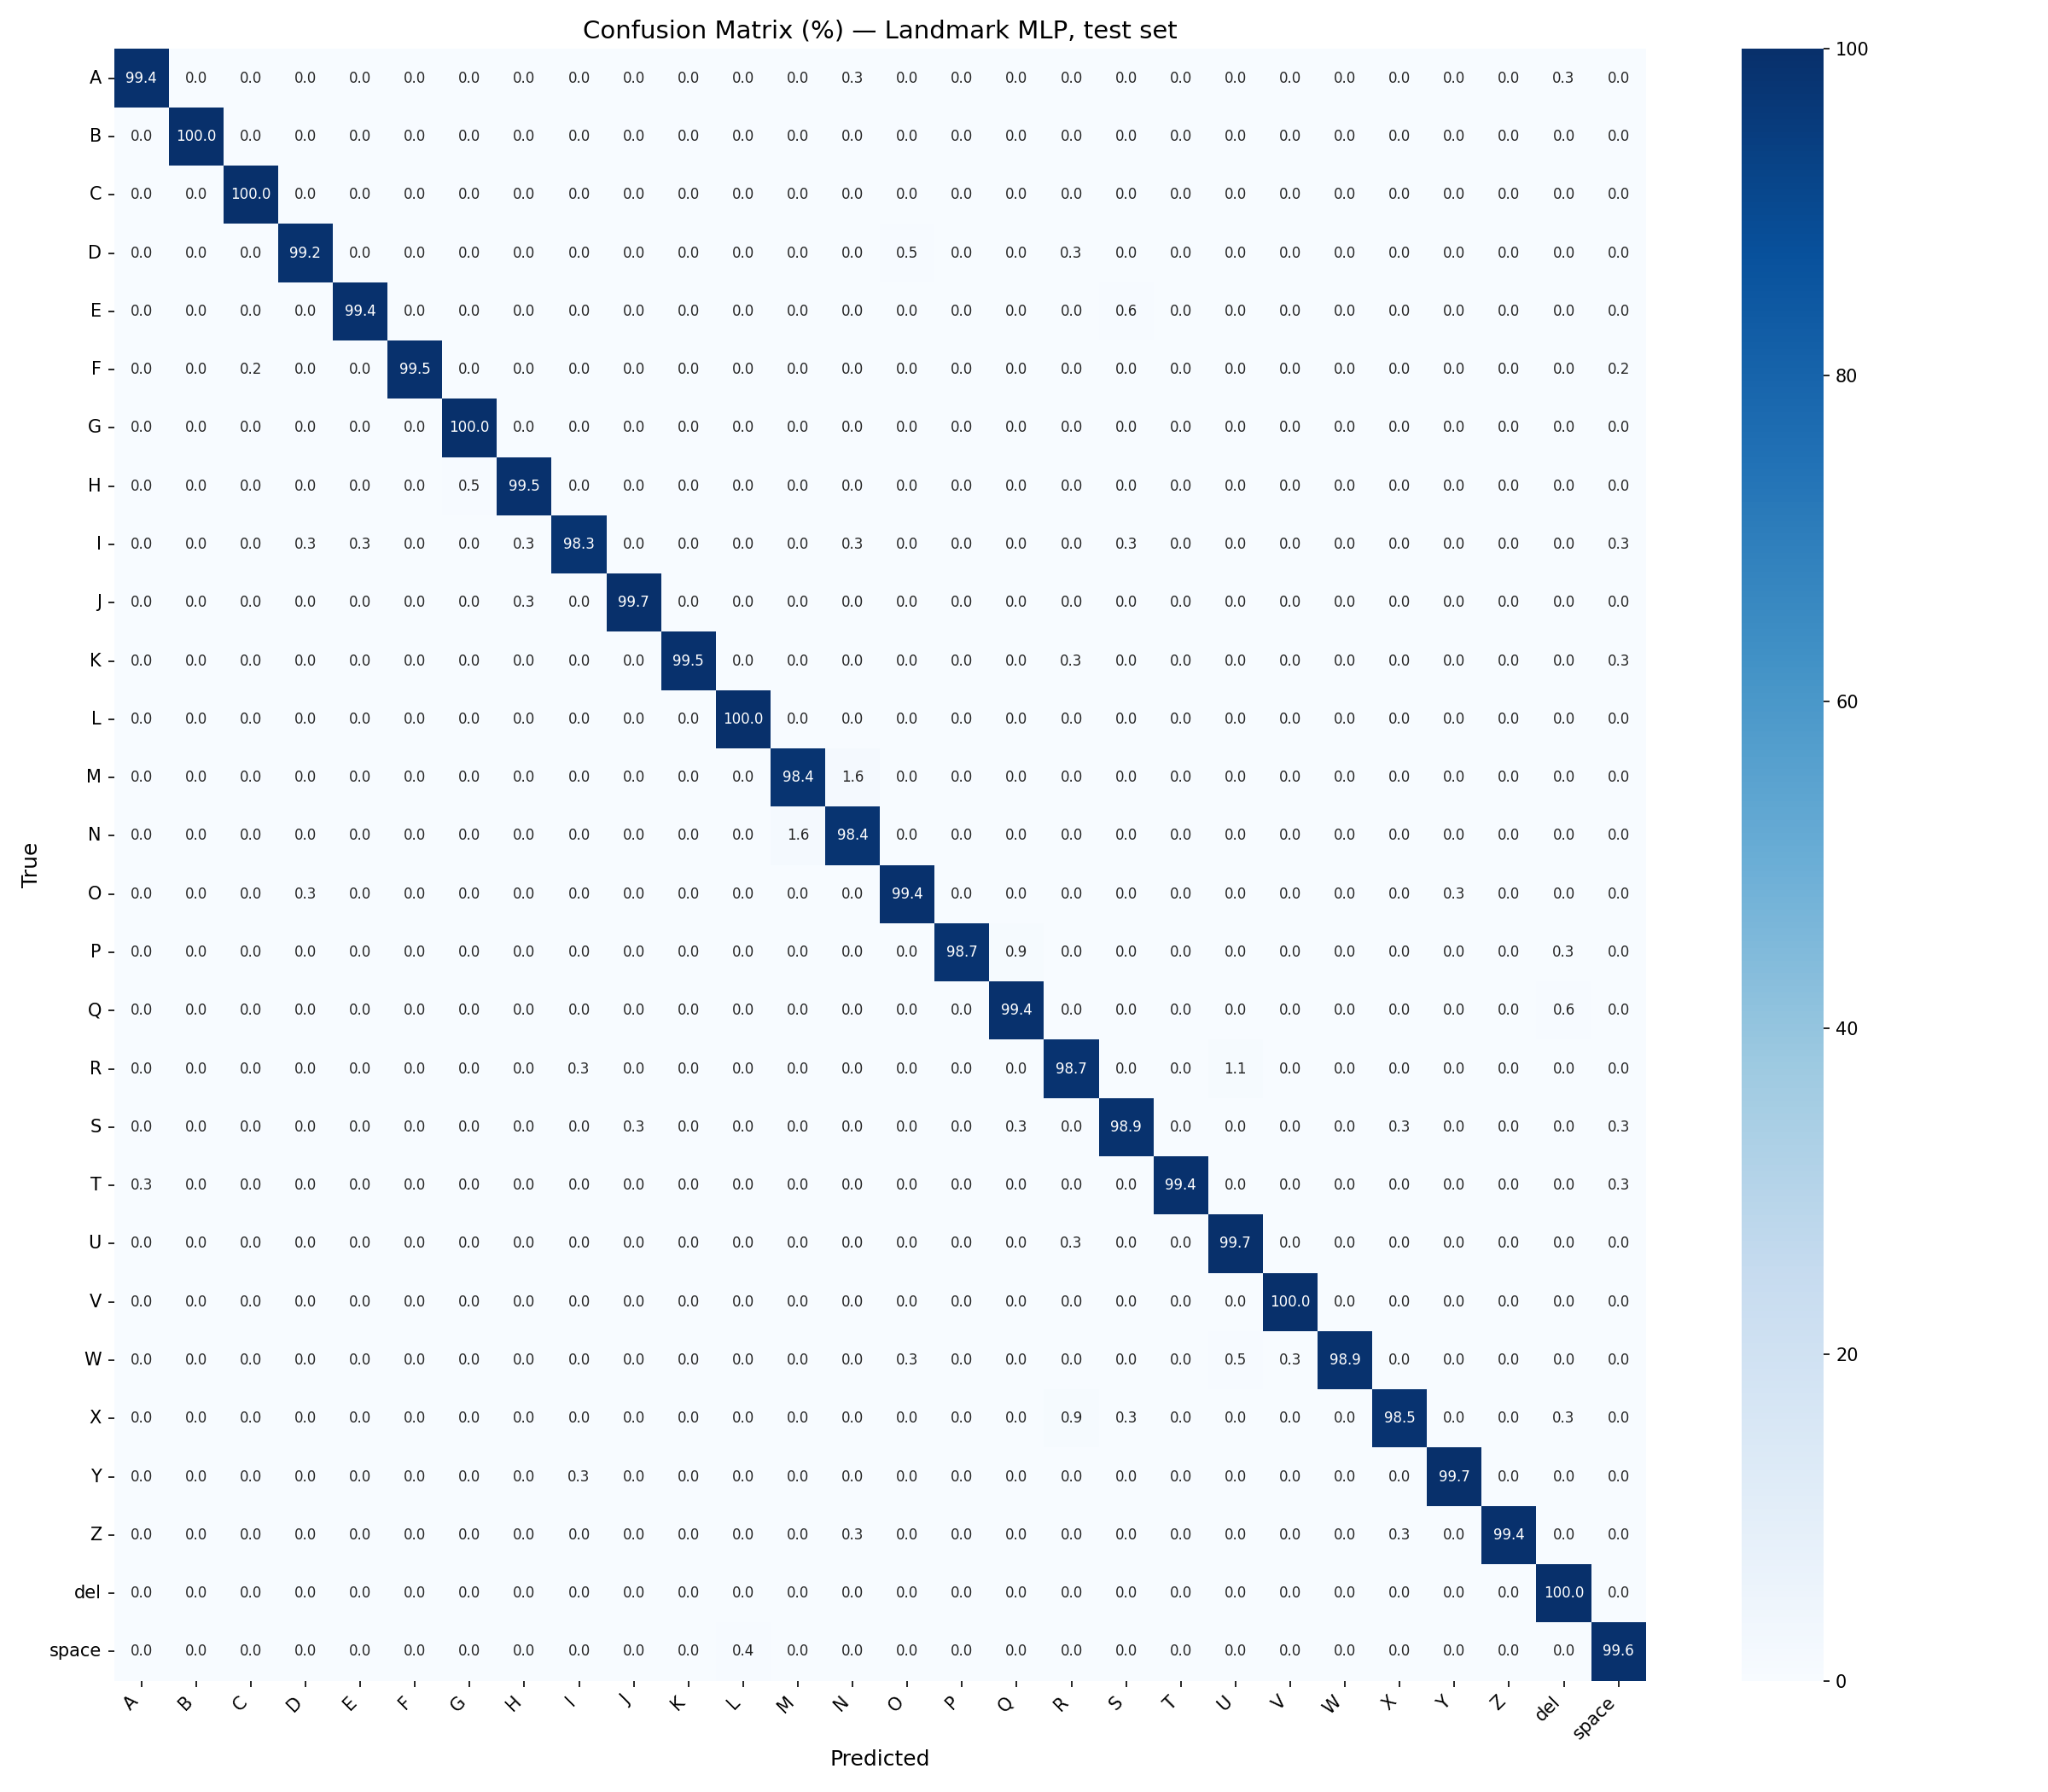
\includegraphics[width=0.9\textwidth]{figures/ch5_cm_mlp_letters.png}
\caption{Row-normalised confusion matrix of the landmark MLP letter
classifier on the detector-recoverable subset of the ASL Alphabet
test partition (73.09\,\% coverage). The matrix is dominated by the
diagonal; off-diagonal cells remain below \SI{2}{\percent} and
concentrate around classes whose handshape MediaPipe captures less
reliably, in particular the thumb-tucked \textit{M}/\textit{N} pair
and the closely related \textit{R}/\textit{U}/\textit{V} group.}
\label{fig:results-cm-mlp}
\end{figure}

Two observations carry over to Chapter~\ref{ch:conclusion}. The first
is that on this dataset the image network is the more reliable choice
because it runs on every input image, whereas the landmark network is
effectively gated on MediaPipe's detection. The 26.91\,\% of test
images on which MediaPipe failed include the entire \texttt{nothing}
class (which contains no hand by construction) and a subset of the
letters~\textit{M} and~\textit{N}, whose thumb-tucked hand-shape
defeats the detector on low-resolution crops. The on-device demo
preserves this asymmetry: the image classifier always produces an
output, while the landmark classifier displays a faded ``no hand
visible'' marker on frames where MediaPipe finds no hand.

The second observation is that the two classifiers occupy opposite
ends of the size/speed trade-off explored in this thesis. The MLP is
65$\times$ smaller and roughly two orders of magnitude faster than
EfficientNet at offline throughput, while losing 0.62 percentage
points of accuracy on the images where it is defined. For practical
mobile deployment, the relevant question is not which of these two
absolute numbers is larger but which configuration is appropriate
under a given resource budget; the on-device measurements of
Section~\ref{sec:results-on-device} answer that question
quantitatively.

A third observation tempers both of the previous ones: the perfect
test accuracy of the image network and the near-perfect accuracy of
the landmark network are not predictions of real-world performance.
Both numbers were obtained on a random split of a single-source
dataset whose images were collected in a controlled setting by a
single contributor on Kaggle. Section~\ref{sec:results-on-device}
reports the substantially noisier behavior of both classifiers when
they are pointed at a new hand under the natural lighting and
background variation of a smartphone camera; the gap between offline
test accuracy and on-device accuracy is the appropriate measure of
how well each model would generalize in production use.

%==============================================================================
\section{Word Recognition Results}
\label{sec:results-words}

The word classifier is evaluated against the five-seed protocol described
in Section~\ref{sec:results-methodology}: five independently trained
BiLSTM instances and a five-seed ensemble that averages their pre-softmax
logits. All six checkpoints are evaluated once on the held-out 201-clip
WLASL-100 test partition. Per-seed scores establish the variance baseline
of the single-model variant; the ensemble line in
Table~\ref{tab:results-words-seeds} is the model that the Android demo
exposes as ``BiLSTM Ensemble (x5)''.

\begin{table}[h]
\centering
\caption{Per-seed and ensemble accuracy on the WLASL-100 test set.}
\label{tab:results-words-seeds}
\begin{tabular}{lccc}
\toprule
\textbf{Model} & \textbf{Top-1 (\%)} & \textbf{Top-5 (\%)} & \textbf{Macro F1} \\
\midrule
BiLSTM seed 0           & 53.23 & 80.60 & 0.491 \\
BiLSTM seed 1           & 52.74 & 78.11 & 0.495 \\
BiLSTM seed 2           & 56.22 & 79.10 & 0.524 \\
BiLSTM seed 3           & 49.75 & 77.61 & 0.447 \\
BiLSTM seed 4           & 48.76 & 79.60 & 0.469 \\
\midrule
Five-seed mean          & 52.14 & 79.00 & 0.485 \\
Five-seed range         & $\pm$3.73 & $\pm$1.49 & $\pm$0.038 \\
\midrule
\textbf{Ensemble (logit avg.)} & \textbf{56.22} & \textbf{81.09} & \textbf{0.521} \\
\bottomrule
\end{tabular}
\end{table}

The training trajectory underlying these numbers is reported in
Figure~\ref{fig:results-lc-lstm}. All five seeds follow the same
overall shape: a steep loss drop and accuracy climb during the
first roughly forty epochs, followed by a long tail of slow
improvement. Seed-to-seed variance is visible throughout but
narrows in the second half of training as the curves converge
toward the band centred on the five-seed mean. Two of the five
seeds triggered the early-stopping criterion before epoch~100,
which is why the per-seed lines terminate at different epochs.
The smoother bold curve is the mean across the overlapping epoch
range and corresponds to the average single-seed trajectory whose
endpoint matches the per-seed mean of
Table~\ref{tab:results-words-seeds}.

\begin{figure}[h]
\centering
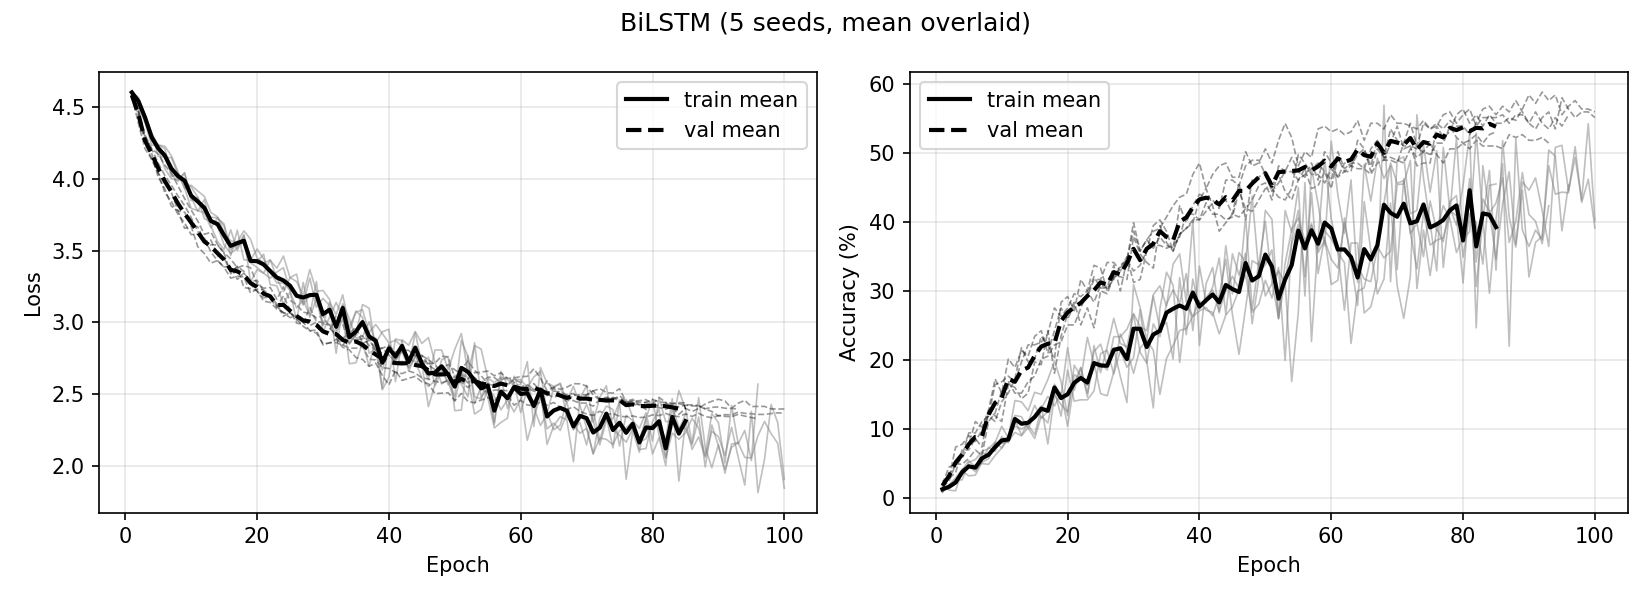
\includegraphics[width=\textwidth]{figures/ch5_lc_lstm.png}
\caption{Training trajectories of the five BiLSTM seeds trained
under the V2 configuration. Thin grey lines are individual seeds,
the bold black lines are the per-epoch mean across seeds (averaged
over the epoch range on which all seeds were still active).}
\label{fig:results-lc-lstm}
\end{figure}

The single-seed Top-1 accuracy varies by roughly four percentage points
across the five runs, which is consistent with the limited test
partition size of 201 clips: a single misclassification moves Top-1 by
0.50 points, so seed-level variance of $\pm 3$--$4$ points is expected
rather than alarming. The ensemble lifts Top-1 from 52.14\,\% (the
five-seed mean) to 56.22\,\% and Top-5 from 79.00\,\% to 81.09\,\%, in
line with the textbook expectation that averaging decorrelated
predictors increases accuracy at the cost of a proportional increase in
inference compute~\cite{dietterich2000ensemble}. Equally important, the
ensemble matches the best single seed exactly on Top-1: the seed~2 run
also reaches 56.22\,\%, but on a different subset of the test clips
than the ensemble, so the two methods do not produce identical predictions.

\subsection{Comparison with Proposal Acceptance Criteria}
\label{sec:results-words-acceptance}

The project proposal defines two thresholds for the word task: a hard
acceptance criterion of Top-1 $\geq 40\,\%$ and a stretch target of
Top-1 $\geq 60\,\%$ on the same test partition. The ensemble result of
56.22\,\% clears the acceptance criterion by 16.22 percentage points
and reaches within 3.78 percentage points of the stretch target. The
gap to the stretch target is consistent with the validation accuracy
of 60.08\,\% reported in Section~\ref{sec:impl-lstm-ensemble}: the
ensemble crosses 60\,\% on the validation set but loses approximately
four points on the smaller and more variable test set, which is the
common pattern observed across deep-learning evaluations on
limited-size data.

\subsection{Position in the WLASL-100 Literature}
\label{sec:results-words-literature}

Table~\ref{tab:results-wlasl-lit} places the ensemble's 56.22\,\% Top-1
against published results on the same WLASL-100 split. The comparison
is necessarily approximate because reported numbers use different
input modalities, preprocessing pipelines and hardware budgets;
nevertheless, the table communicates the relative position of a
hands-only landmark model among the available approaches.

\begin{table}[h]
\centering
\caption{Reported Top-1 accuracy on the WLASL-100 test split. Numbers
are quoted from each publication; the modality column distinguishes
RGB, body pose, body+hand pose and hand-only inputs.}
\label{tab:results-wlasl-lit}
\begin{tabular}{llll}
\toprule
\textbf{Year} & \textbf{Method} & \textbf{Modality} & \textbf{Top-1 (\%)} \\
\midrule
2020 & I3D~\cite{li2020wlasl}              & RGB                & 65.89 \\
2020 & Pose-TGCN~\cite{li2020wlasl}        & Body pose          & 55.43 \\
2020 & VGG-GRU~\cite{li2020wlasl}          & RGB                & 25.97 \\
2020 & TK-3D ConvNet~\cite{li2020transferring} & RGB (+ web news transfer) & 77.55 \\
2021 & Fusion-3~\cite{hosain2021fusion}    & RGB + body pose    & 75.67 \\
2022 & SPOTER~\cite{bohacek2022spoter}     & Body+hand pose     & 63.18 \\
\midrule
\textbf{2026} & \textbf{This work (BiLSTM ensemble)} & \textbf{Hands only} & \textbf{56.22} \\
\bottomrule
\end{tabular}
\end{table}

Two observations frame the result. First, the RGB-based pipelines
operate on a substantially heavier input pipeline---raw video
frames---and produce model sizes that are an order of magnitude
larger than 5.51\,MB. The hands-only configuration sacrifices roughly
10 points of Top-1 accuracy relative to the single-stream I3D baseline,
and just over 20 points against the strongest reported method on
WLASL-100---the cross-domain TK-3D ConvNet of Li et al., which
augments I3D with knowledge transferred from subtitled news
videos---in exchange for a 200~ms inference budget on a phone CPU.
Second, when the comparison is restricted to landmark-only methods,
the result is competitive: the ensemble is within one point of the
body-pose Pose-TGCN baseline and within seven points of the
transformer-based SPOTER, despite using a smaller architecture and a
strictly smaller input feature set (21 hand landmarks per frame,
against 55 upper-body keypoints for Pose-TGCN and 54 head-body-hand
landmarks for SPOTER). The trade-off
characterized in Chapter~\ref{ch:implementation} therefore plays out
as expected on the offline benchmark: heavier RGB or multi-stream
pipelines win on accuracy, lighter landmark pipelines win on
deployability, and the present model occupies an intentional point
on that curve.

\subsection{Inference Latency}
\label{sec:results-words-latency}

Offline inference latency for the BiLSTM single model is
1.87\,ms per sample on the training GPU, corresponding to a throughput
of 534 frames per second on the same hardware. The ensemble inflates
this by approximately a factor of five, in line with the
five-checkpoint structure; on the same GPU the ensemble reaches roughly
110~FPS at an end-to-end latency of 9~ms. Both numbers are well above
the proposal's non-functional requirement of 10~FPS
(NFR-04) on the offline machine. The corresponding on-device numbers,
which include the MediaPipe landmark stage and run on the Android test
phone, are reported in Section~\ref{sec:results-on-device}; they are
the deployment-relevant numbers.

%==============================================================================
\section{Ablation Study}
\label{sec:results-ablation}

The word classifier reported in Section~\ref{sec:results-words} did not
arrive at 56.22\,\% Top-1 in a single step. An earlier configuration
(referred to internally as~V1) was trained with single-hand input,
without sequence-level augmentation and without ensemble averaging; it
reached only 20.00\,\% validation accuracy on the same WLASL-100 split.
The remaining 36 percentage points were gained incrementally over six
modifications which together define the V2 configuration described in
Section~\ref{sec:impl-lstm}. Table~\ref{tab:results-ablation} summarizes
the trajectory and is the single most useful artefact for understanding
which design choices carried the most weight on this dataset.

\begin{table}[h]
\centering
\caption{Incremental ablation from the V1 baseline to the V2 ensemble.
Validation accuracy is reported because the test set was kept frozen
until the final V2 configuration had been selected; the bottom row
reports the corresponding test accuracy that
Section~\ref{sec:results-words} discusses in detail.}
\label{tab:results-ablation}
\begin{tabular}{clcc}
\toprule
\textbf{Step} & \textbf{Added component} & \textbf{Val Top-1 (\%)} & \textbf{$\Delta$} \\
\midrule
0 & V1 baseline (single hand, no augmentation)        & 20.00 & --- \\
1 & + WLASL \texttt{frame\_start}/\texttt{frame\_end} crop & (bundled) & (bundled) \\
2 & + two-hand extraction with presence flags         & (bundled) & (bundled) \\
3 & + sequence augmentation\textsuperscript{a}        & 47.33     & +27.33 \\
4 & + mixup ($\alpha=0.2$)                            & (bundled) & (bundled) \\
5 & + hidden size 128 $\rightarrow$ 192               & (bundled) & (bundled) \\
6 & + time-scaling $\pm 20\,\%$                       & (bundled) & (bundled) \\
7 & + \texttt{WeightedRandomSampler}                  & 54.32 & +6.99 \\
8 & + mixup $\alpha$ 0.2 $\rightarrow$ 0.4            & 58.85 & +4.53 \\
9 & + five-seed ensemble (logit averaging)            & \textbf{60.08} & +1.23 \\
\midrule
\multicolumn{2}{l}{\textbf{Test set (V2 ensemble)}}    & \multicolumn{2}{c}{\textbf{56.22 / 81.09 (Top-1 / Top-5)}} \\
\bottomrule
\end{tabular}
\\[0.4em]
\footnotesize\textsuperscript{a}Temporal jitter $\pm 4$ frames, frame dropout $p{=}0.15$, Gaussian noise $\sigma{=}0.02$.
\end{table}

Steps~1--6 were applied as a single ``data and architecture'' bundle
during V2 development, so the table reports the marginal effect of the
bundle (step~3, +27.33 points) rather than that of each individual
component. The decision to bundle these modifications was deliberate:
each one targets a different failure mode of V1 (frame-window noise,
missing second hand, identical input sequences across epochs,
underparameterized recurrent state, fixed-length sampling) and
isolating them would have multiplied the training budget for a
question that the proposal does not require us to answer. A finer
component-level ablation is listed as future work in
Chapter~\ref{ch:conclusion}.

The remaining three rows isolate single decisions and warrant separate
comment. The \texttt{WeightedRandomSampler} (step~7, +6.99 points)
re-balances the loss against the long tail of WLASL-100, where the
majority of words have between one and four training clips; without
this sampler the model collapses onto the head classes and the macro
F1 score drops noticeably even when Top-1 stays competitive. Increasing
the mixup intensity from $\alpha = 0.2$ to $\alpha = 0.4$ (step~8,
+4.53 points) increases the regularization pressure and is what closed
most of the remaining single-seed gap to the proposal stretch target;
the choice was guided by the validation curves, which showed the
$\alpha = 0.2$ run beginning to overfit around epoch 60. The five-seed
ensemble (step~9, +1.23 points on the validation set and +4.08 points
relative to the five-seed mean of 52.14\,\% on the test set, as
discussed in Section~\ref{sec:results-words}) is the cheapest source of
accuracy in the entire pipeline---the additional cost is purely at
inference time and is bounded by the five-fold latency penalty
quantified in Section~\ref{sec:results-on-device}.

%==============================================================================
\section{Error Analysis}
\label{sec:results-errors}

A model that reaches 56.22\,\% Top-1 also misclassifies 43.78\,\% of
the WLASL-100 test clips. Whether those errors are random or
structured is the more interesting question and is what this section
addresses. Figure~\ref{fig:results-cm-words} visualises the
ensemble's row-normalised confusion matrix on the 25 most populous
classes of the WLASL-100 test partition; the remaining 75 classes
each contribute at most a single test clip and are omitted to keep
the matrix legible. The matrix is dominated by a clear diagonal,
with the two visible off-diagonal cells (\texttt{woman}\,$\to$\texttt{fine},
\texttt{last}\,$\to$\texttt{before}) corresponding to signs that
share location or motion with their misclassified target. The
matrix of the ensemble was inspected systematically for the
five most frequent confusion pairs across the full 100-class
matrix; the result is summarised in
Table~\ref{tab:results-confusions}. None of the five pairs are random.
Each one corresponds to a pair of ASL signs that share a handshape, a
location on the body or a movement trajectory, and the model's mistakes
therefore look like the mistakes a beginning ASL student would make
rather than like the noise of an under-trained network.

\begin{table}[h]
\centering
\caption{Five most frequent confusion pairs in the ensemble predictions,
with the linguistic reason for the visual ambiguity.}
\label{tab:results-confusions}
\begin{tabular}{llp{7.4cm}}
\toprule
\textbf{Ground truth} & \textbf{Prediction} & \textbf{Reason for visual similarity} \\
\midrule
\texttt{black}  & \texttt{who}   & Both one-handed; index-finger motion near the head and cheek. \\
\texttt{dog}    & \texttt{later} & Both one-handed; finger-snap motion with the same handshape transition. \\
\texttt{change} & \texttt{how}   & Both two-handed; rotating-fist handshape with bilateral movement. \\
\texttt{want}   & \texttt{many}  & Both two-handed; fingers open from a closed configuration. \\
\texttt{mother} & \texttt{fine}  & 5-handshape with thumb contact on chin or forehead in both signs. \\
\bottomrule
\end{tabular}
\end{table}

\begin{figure}[h]
\centering
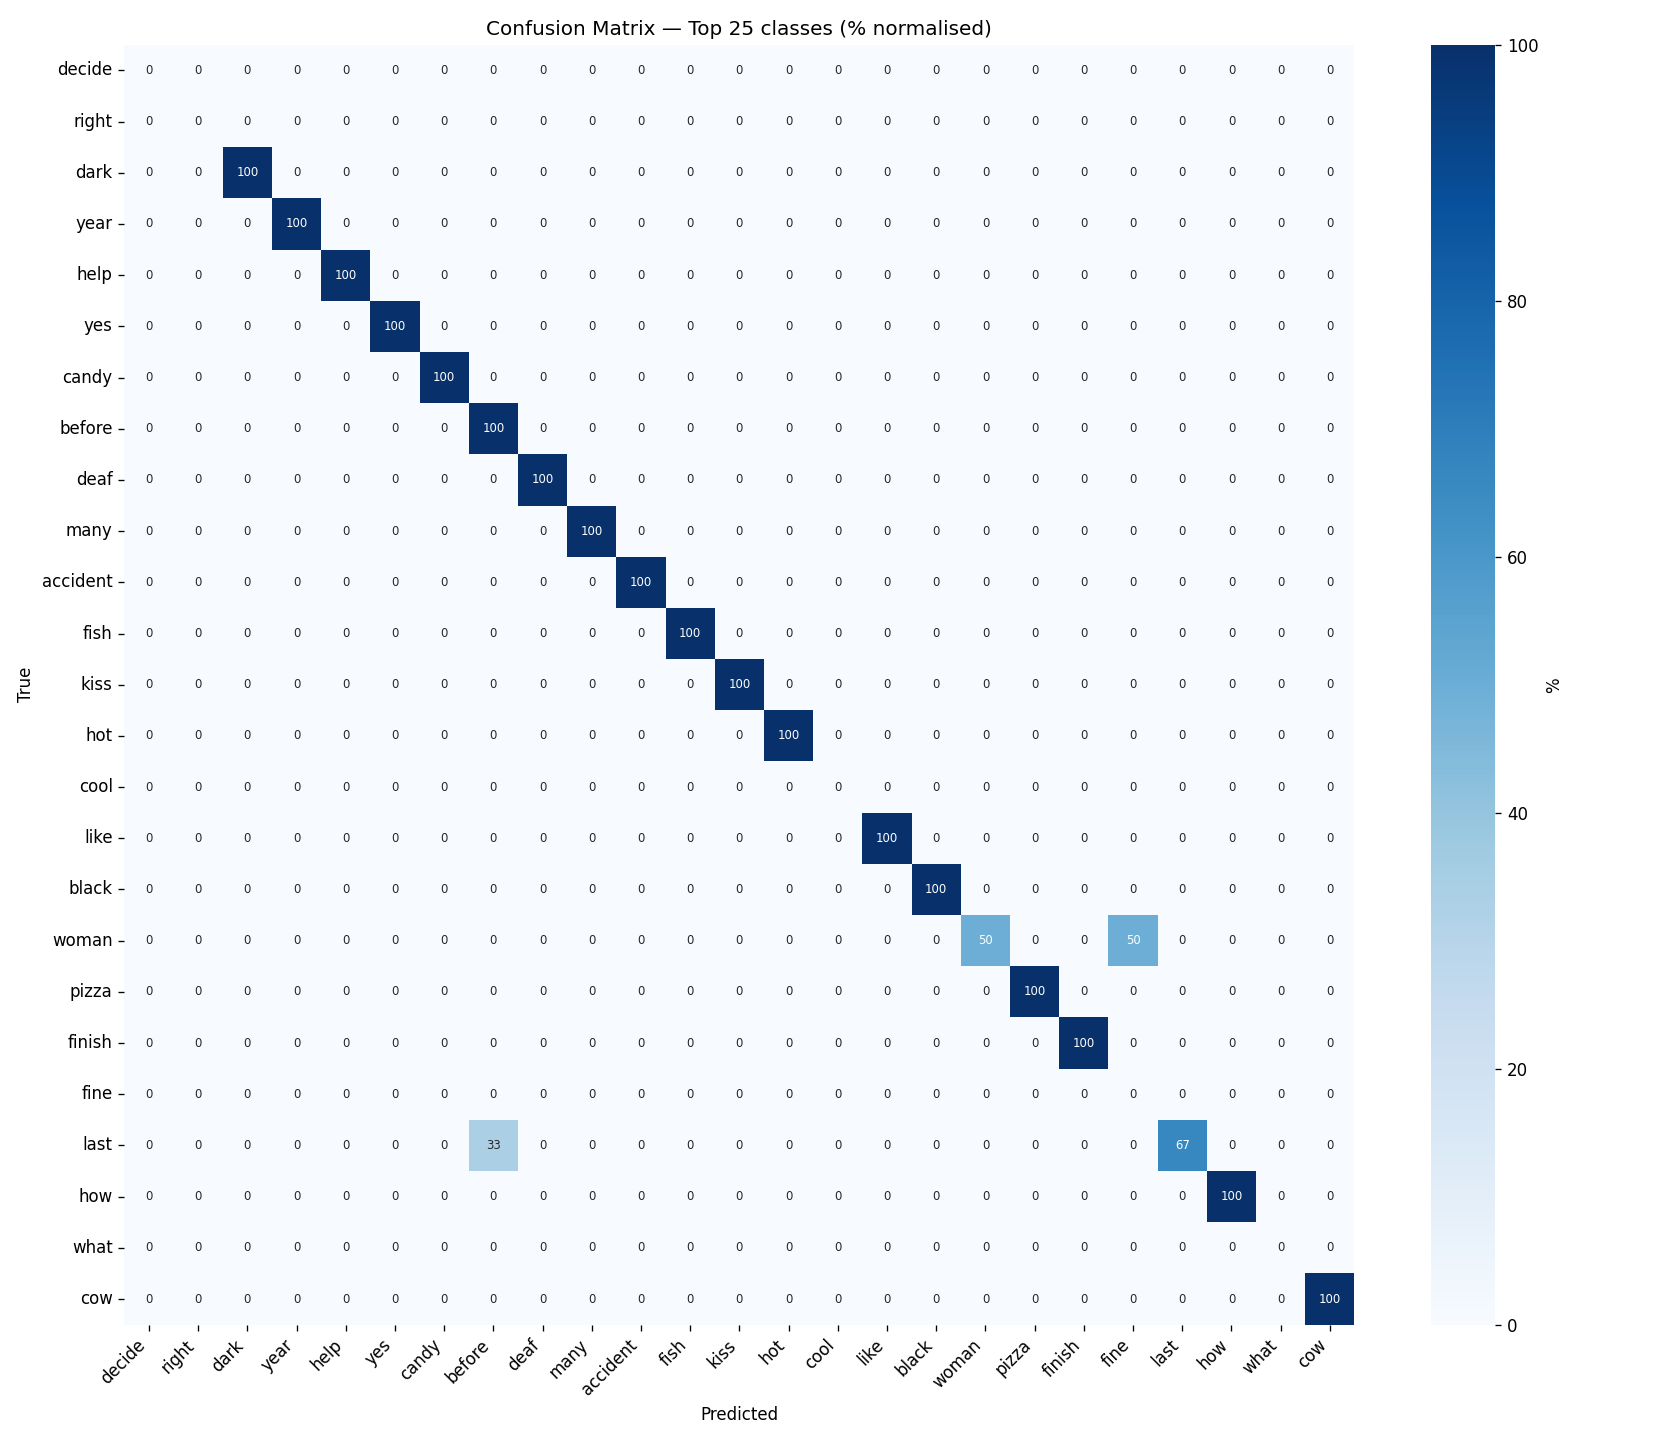
\includegraphics[width=\textwidth]{figures/ch5_cm_lstm_words.png}
\caption{Row-normalised confusion matrix of the five-seed BiLSTM
ensemble on the 25 most populous classes of the WLASL-100 test
partition. The full 100-class matrix is dominated by single-clip
rows that are not visually informative; the truncation to the top
25 classes by test support preserves the diagonal-with-isolated-confusions
structure of the prediction error.}
\label{fig:results-cm-words}
\end{figure}

The implication of the table is that the model has internalized the
high-level structure of an ASL sign (handedness, location and the
class of movement) and fails on the fine-grained handshape or
trajectory details that distinguish minimally different signs. From a
sign-language-linguistic perspective this is the expected failure
mode of a hands-only model: pose information about the arm and torso
would resolve several of these confusions, and facial markers would
resolve others (the distinction between \texttt{mother} and
\texttt{fine}, in particular, is partly tied to a facial component
that hand landmarks cannot capture). The Limitations subsection of
Chapter~\ref{ch:conclusion} returns to this point in the context of
multi-stream models that combine hand, body and facial input.

Two structural caveats round out the error picture. First, two of the
hundred WLASL-100 classes (\texttt{later} and \texttt{book}) have
\emph{zero} examples in the official test partition because the
canonical split allocates their few available clips to train and
validation. The macro F1 score of 0.521 reported in
Table~\ref{tab:results-words-seeds} therefore averages over the
98~effective classes that have at least one test clip, rather than
over the full 100. This is a property of the WLASL-100 evaluation
protocol, not of the model. Second, the Top-5 accuracy of 81.09\,\%
combined with a Top-1 accuracy of 56.22\,\% means that the correct
label is among the top five predictions in roughly 25 percentage
points of clips that the Top-1 metric counts as failures. In a
real-world interactive application this gap is recoverable through a
``did you mean'' interaction surface (a confidence-ranked shortlist of
candidate signs); the Android demo of Chapter~\ref{ch:implementation}
does not implement such a surface but the option is preserved for
future work.

%==============================================================================
\section{On-Device Performance}
\label{sec:results-on-device}

The offline numbers reported in
Sections~\ref{sec:results-letters}--\ref{sec:results-words} are measured
on the training GPU and are useful for cross-checking the model against
the published literature, but they do not characterise the system that
the proposal actually promised to deliver: an Android application that
runs the classifiers on-device, displays the recognised letter or word
and reports its own throughput and latency. This section reports the
on-device counterparts of those numbers, measured directly on two
mid-tier Android phones during the manual test described in
Section~\ref{sec:results-qualitative}.

\subsection{Test Devices and Protocol}
\label{sec:results-on-device-protocol}

Two phones were used in the manual test. The first, a
\textbf{TECNO~SPARK 20C}, is an entry-level device built around a
MediaTek Helio~G36 SoC (8\,nm, 8 ARM Cortex-A53 cores at up to
\SI{2.2}{\giga\hertz}, 8\,GB RAM, Android~13). It represents the
budget segment of the Android market on which an accessibility tool
must remain usable. The second, a \textbf{Xiaomi~15T~Pro}, is a
2025-generation flagship built around a MediaTek Dimensity~9400+ SoC
(3\,nm, 1+3+4 cluster topology with an ARM Cortex-X925 prime core,
12\,GB LPDDR5X RAM, Android~15) and represents the upper end of the
deployable hardware. Both devices ran the same APK
(\texttt{./gradlew installDebug}, commit \texttt{b1d5465} plus the
Words single-shot lock changes of Section~\ref{sec:impl-android-pipeline})
under matched conditions: daylight illumination from a window, a
neutral background, and a hand-to-camera distance of
\SIrange{30}{50}{\centi\metre}. Battery Saver was disabled on both
devices to prevent CPU throttling from contaminating the measurement.

For each of the four classifiers, the relevant tab of the application
was opened, a static target (a single letter for the letter models, a
single fixed word for the word models) was held in front of the camera
for \SI{60}{\second}, and the on-screen FPS and latency badges were
read every ten seconds from a screen recording, producing six samples
per model and device. The badge reports the end-to-end pipeline
latency measured inside the analyzer: camera frame
$\rightarrow$ MediaPipe Hands $\rightarrow$ classifier
$\rightarrow$ UI publication. It is therefore the deployment-relevant
quantity, not an isolated model-inference number. To avoid a
device-mismatch confound the letter models were measured on both
phones; the word models were measured on both phones initially, but
on the TECNO the ensemble produced latencies that made the application
unusable (Section~\ref{sec:results-on-device-words}), so the Words
qualitative test of Section~\ref{sec:results-qualitative} was carried
out exclusively on the Xiaomi.

\subsection{Letter Models}
\label{sec:results-on-device-letters}

Table~\ref{tab:on-device-letters} reports the six-sample mean,
minimum and maximum FPS and latency for the two letter classifiers on
both devices. Two patterns emerge clearly. On the Xiaomi 15T~Pro both
classifiers saturate the camera at \SI{30}{FPS} with latencies well
inside the proposal's non-functional budget (NFR-04, \SI{10}{FPS}
end-to-end on the offline machine). On the TECNO SPARK~20C only the
landmark MLP keeps the pipeline within a real-time budget; the
image-based EfficientNet stays at a respectable \SI{20.7}{FPS}
average, but the end-to-end latency rises to \SI{203}{ms} mean and
peaks at \SI{220}{ms}, an order of magnitude higher than its Xiaomi
counterpart.

\begin{table}[h]
\centering
\caption{On-device throughput and latency of the two letter
classifiers, measured from the in-app FPS/latency badge over a
60-second window (six samples per cell).}
\label{tab:on-device-letters}
\resizebox{\textwidth}{!}{%
\begin{tabular}{llccccc}
\toprule
\textbf{Model} & \textbf{Device} & \textbf{Mean FPS} & \textbf{Min FPS} & \textbf{Max FPS} & \textbf{Mean lat.\ (ms)} & \textbf{Max lat.\ (ms)} \\
\midrule
EfficientNet-B0 & Xiaomi 15T Pro   & 30.0 & 30 & 30 & 35.2 & 40 \\
EfficientNet-B0 & TECNO SPARK 20C  & 20.7 & 18 & 24 & 203.3 & 220 \\
Landmark MLP    & Xiaomi 15T Pro   & 30.0 & 30 & 30 & 18.7 & 25 \\
Landmark MLP    & TECNO SPARK 20C  & 24.5 & 24 & 25 & 21.7 & 30 \\
\bottomrule
\end{tabular}%
}
\end{table}

The relative behaviour of the two letter classifiers on the entry-level
TECNO is the more informative result. The landmark MLP, whose
checkpoint is only \SI{0.24}{MB} (Table~\ref{tab:results-letters}),
adds approximately \SI{4}{ms} to the MediaPipe baseline and stays
within \SI{30}{ms} maximum end-to-end latency on the same hardware on
which EfficientNet-B0 needs \SI{200}{ms}. The image classifier
therefore pays the entire on-device cost difference in latency rather
than in dropped frames: the camera continues to deliver at roughly
\SI{20}{FPS}, but each frame's prediction lags the visible hand by a
fifth of a second. For static fingerspelling this lag does not affect
the correctness of the displayed label (the manual test of
Section~\ref{sec:results-qualitative} confirms this) but for any
gesture that involves motion it would be visible.

\subsection{Word Models}
\label{sec:results-on-device-words}

Table~\ref{tab:on-device-words} reports the equivalent measurements
for the two word classifiers. On the Xiaomi the single-model variant
runs at \SI{30}{FPS} with a mean end-to-end latency of \SI{31.7}{ms};
the five-seed ensemble inflates the model-inference component by the
expected factor of approximately five, raising mean latency to
\SI{80}{ms} but leaving the camera-driven FPS unchanged. Both
configurations are comfortably within an interactive budget on the
flagship hardware.

\begin{table}[h]
\centering
\caption{On-device throughput and latency of the two word
classifiers (six samples per cell). The TECNO entry for the ensemble
is the headline result of this section: a five-fold latency
inflation that is invisible on flagship hardware becomes
interaction-breaking on the entry-level SoC.}
\label{tab:on-device-words}
\resizebox{\textwidth}{!}{%
\begin{tabular}{llccccc}
\toprule
\textbf{Model} & \textbf{Device} & \textbf{Mean FPS} & \textbf{Min FPS} & \textbf{Max FPS} & \textbf{Mean lat.\ (ms)} & \textbf{Max lat.\ (ms)} \\
\midrule
BiLSTM single   & Xiaomi 15T Pro   & 30.0 & 30 & 30 &  31.7 &  40 \\
BiLSTM single   & TECNO SPARK 20C  & 22.0 & 20 & 24 & 201.7 & 215 \\
BiLSTM ensemble & Xiaomi 15T Pro   & 30.0 & 30 & 30 &  80.0 &  90 \\
BiLSTM ensemble & TECNO SPARK 20C  & 17.0 & 14 & 22 & 665.0 & 700 \\
\bottomrule
\end{tabular}%
}
\end{table}

On the TECNO the picture changes qualitatively. The single-model
variant produces \SI{200}{ms} mean latency in the same range as
EfficientNet-B0 on the same device, and the ensemble inflates this
fivefold to a mean of \SI{665}{ms} with a peak of \SI{700}{ms}.
Because the Words pipeline collects a 32-frame buffer before
inference (Section~\ref{sec:impl-android-pipeline}), a latency in
this range means that the prediction for a sign arrives roughly two
thirds of a second after the user has finished producing it; the
single-shot lock then holds that label until the hand-down release
fires. In practice this combination is unusable: the user has to
hold the sign motionless for an unnatural duration and the system
feels disconnected from the input. The Xiaomi was added to the test
plan precisely to side-step this confound and obtain a clean reading
of the word classifiers' accuracy (Section~\ref{sec:results-qualitative})
on hardware where the latency does not corrupt the user's behavior.

\subsection{Why CPU Execution on the Entry-Level SoC}
\label{sec:results-on-device-cpu}

The asymmetry between the two devices is not a pure consequence of
raw SoC performance. During early on-device testing the TFLite GPU
delegate was evaluated for the image and LSTM classifiers. The
delegate produced a long initial warm-up (over a second on the
TECNO) and, more importantly, was implicated in a recurring
\texttt{MediaPipeException: smaller timestamp than processed
timestamp} crash on cold start, where MediaPipe's
\texttt{LIVE\_STREAM} mode received non-monotonic timestamps from
the first few frames after the camera bound to the analyzer. The
fix selected for the deployed build was to drop the GPU delegate
and run all four classifiers on the CPU through XNNPACK, with a
volatile guard on the last sent timestamp and a try/catch around
\texttt{detectAsync}. This decision trades a measurable amount of
peak throughput on supported devices for a build that never crashes
in the cold-start path.

Table~\ref{tab:on-device-letters} and
Table~\ref{tab:on-device-words} are therefore not measurements of an
intrinsic ``ARM phone'' limit; they measure CPU execution of the
classifiers on the two devices' respective CPU clusters. The
Dimensity~9400+ absorbs the cost of CPU-only execution invisibly,
while the Helio~G36 does not. The same decision (stability over
peak speed) thus has an \emph{asymmetric} cost across the hardware
spectrum, which is the precise observation that
Section~\ref{sec:conclusion-limitations} returns to as the
performance-side limitation of the delivered system.

\subsection{Decision Matrix for Mobile Deployment}
\label{sec:results-on-device-matrix}

Combining the on-device throughput and latency reported in this
section with the accuracy numbers of the previous sections produces
a simple deployment guideline. On an entry-level SoC (Helio~G36 or
comparable) only the landmark MLP delivers an interactive
experience; the image classifier remains correct but loses
responsiveness, the BiLSTM single model is borderline, and the
ensemble is not usable. On a mid-range or flagship SoC
(Dimensity~9400+ or comparable) all four classifiers meet their
budgets and the choice between them collapses back to the
accuracy/size trade-off captured in
Tables~\ref{tab:results-letters} and~\ref{tab:results-words-seeds}.
This device-conditional model selection is the most concrete
operational outcome of the thesis and is the headline argument for
including a landmark MLP variant on the letter task at all.

%==============================================================================
\section{Real-Device Qualitative Evaluation}
\label{sec:results-qualitative}

The on-device performance numbers of the previous section answer
\emph{how fast} the classifiers run on a phone; this section answers
\emph{how often they are right} on a phone, under naturalistic
camera conditions that are systematically out-of-distribution
relative to the offline test partitions of
Sections~\ref{sec:results-letters} and~\ref{sec:results-words}. The
purpose of the experiment is not to produce a new accuracy number to
compete with the offline results---a single human signer cannot
sample the variation of the underlying populations---but to verify
that the proposal's qualitative criterion (``the recognised letter or
word is written to the screen'') is satisfied in real use, and to
characterise where the offline numbers are misleading.

\subsection{Protocol}
\label{sec:results-qualitative-protocol}

A single test user (the author) produced one trial per class for
each classifier under each device condition. For the letter
classifiers, this is 29 trials per (model, device) cell, of which 28
are measurable: the \texttt{nothing} class cannot be evaluated under
the deployed pipeline because the analyzer does not invoke the
classifier when MediaPipe Hands fails to detect a hand. For the
word classifiers, this is 100 trials per model, covering the full
WLASL-100 vocabulary in the order of the canonical
\texttt{gloss\_to\_idx.json} mapping. Each trial recorded the Top-1
label, the Top-1 confidence from the in-app panel, and, when the
Top-1 was wrong, whether the correct label appeared in the Top-3
panel as well as which incorrect label the model produced.

Two procedural rules apply throughout. First, the canonical
fingerspelling pose of each letter was held for three seconds
before the panel value was recorded, so that the single-shot lock
of Section~\ref{sec:impl-android-pipeline} settled. Second, on the
Words tab the per-trial behaviour follows the new lock state
machine described in Section~\ref{sec:impl-android-pipeline}: if
the user noticed an erroneous start \emph{before} the buffer
filled they could lower the hand and re-attempt, but once the
buffer fill completed and a prediction was latched the trial was
counted as taken. This rule prevents the protocol from collapsing
into a best-of-many test that would over-state real-world accuracy.

\subsection{Letter Models, Device-by-Device}
\label{sec:results-qualitative-letters}

Table~\ref{tab:qual-letters} reports the manual-test accuracy of the
two letter classifiers on both phones over their 28 measurable
classes. Three observations frame the result.

\begin{table}[h]
\centering
\caption{Manual-test accuracy of the two letter classifiers across
both devices. The 28 measurable classes exclude the
\texttt{nothing} class, which the deployed pipeline does not
classify by design.}
\label{tab:qual-letters}
\begin{tabular}{llcccc}
\toprule
\textbf{Model} & \textbf{Device} & \textbf{Top-1 (\%)} & \textbf{Top-3 (\%)} & \textbf{Mean conf.\ (\%)} \\
\midrule
EfficientNet-B0 & TECNO SPARK 20C  &  92.9 (26/28) & 100.0 & 94.7 \\
EfficientNet-B0 & Xiaomi 15T Pro   & 100.0 (28/28) & 100.0 & 98.2 \\
Landmark MLP    & TECNO SPARK 20C  & 100.0 (28/28) & 100.0 & 99.6 \\
Landmark MLP    & Xiaomi 15T Pro   & 100.0 (28/28) & 100.0 & 100.0 \\
\bottomrule
\end{tabular}
\end{table}

First, the gap between offline test accuracy and on-device accuracy
is small for both classifiers. EfficientNet-B0 drops from
\SI{100}{\percent} on the offline test partition to \SI{92.9}{\percent}
on the TECNO and remains at \SI{100}{\percent} on the Xiaomi; the
landmark MLP drops from \SI{99.38}{\percent} offline to a uniform
\SI{100}{\percent} on both devices. The single-user OOD penalty that
Section~\ref{sec:results-letters} flagged as the appropriate yardstick
for production readiness is therefore at most seven percentage points
on the worst-case (device, model) cell and zero on three of the four
cells. This is the empirical evidence behind the chapter's claim that
the letter classifiers are deployment-ready.

Second, the two errors observed on the TECNO with EfficientNet-B0
were both image-pipeline mistakes rather than handshape
ambiguities: D was classified as K or R with \SI{60}{\percent}
confidence and K was classified as W with \SI{40}{\percent}
confidence. The same hand pose produced clean predictions on the
Xiaomi with EfficientNet (D at \SI{90}{\percent}, K at
\SI{85}{\percent} confidence). The landmark MLP did not produce these
errors on either device. This is the inverse of the offline result:
in the offline partition the image network was the more accurate
classifier (\SI{100}{\percent} vs \SI{99.38}{\percent}); in real
deployment on a budget phone, it is the less accurate of the two.
The most plausible explanation is that the MediaPipe landmark
abstraction discards exactly the camera-pipeline noise (sharper or
softer image-signal processing, white-balance shifts, slight blur)
to which a pixel-based network is sensitive; the same observation
underlies the literature consensus on pose-based models for
on-device sign recognition.

Third, neither classifier degraded gracefully on the
\texttt{nothing} class because the deployed pipeline does not
attempt to classify it---the analyzer simply does not invoke the
classifier when MediaPipe Hands reports an empty frame. This is the
correct behaviour for an interactive application (no spurious
predictions when the user's hand is not on screen), but it means the
on-device evaluation cannot report a number for that class and the
offline test partition remains the appropriate ground truth for the
``no hand'' negative.

\subsection{Word Models on the Xiaomi}
\label{sec:results-qualitative-words}

Table~\ref{tab:qual-words} reports the manual-test accuracy of the
two word classifiers across the full WLASL-100 vocabulary on the
Xiaomi. Because the TECNO ensemble latency made trials unproductive
(Section~\ref{sec:results-on-device-words}), Words trials on the
TECNO are not reported.

\begin{table}[h]
\centering
\caption{Manual-test accuracy of the two word classifiers on the
WLASL-100 vocabulary (100 trials per model, one trial per class)
on the Xiaomi 15T Pro. Mean Top-1 confidence is computed over the
correctly classified subset.}
\label{tab:qual-words}
\begin{tabular}{lcccc}
\toprule
\textbf{Model} & \textbf{Top-1 (\%)} & \textbf{Top-3 (\%)} & \textbf{Mean conf.\ (\%)} \\
\midrule
BiLSTM single                & 38.0 & 71.0 & 32.0 \\
BiLSTM ensemble (x5)         & 49.0 & 72.0 & 29.1 \\
\midrule
$\Delta$ (Ensemble $-$ Single) & $+11.0$ & $+1.0$ & $-2.9$ \\
\bottomrule
\end{tabular}
\end{table}

The single-model variant reached \SI{38.0}{\percent} Top-1 against
its offline test number of \SI{52.14}{\percent} (the five-seed
mean of Table~\ref{tab:results-words-seeds}); the ensemble reached
\SI{49.0}{\percent} against its offline test number of
\SI{56.22}{\percent}. The single-user OOD gap for the word
classifier is therefore \SI{14}{\percent} points (single) and
\SI{7}{\percent} points (ensemble), which is the order of magnitude
the proposal anticipated when it set the manual-test acceptance
threshold to \SI{35}{\percent} for the single model and
\SI{40}{\percent} for the ensemble. Both thresholds were cleared,
the latter by nine percentage points.

Two structural observations are worth recording. The first is the
shape of the ensemble improvement: it adds eleven Top-1 points
(\SI{38.0}{\percent}~$\rightarrow$~\SI{49.0}{\percent}) but only one
Top-3 point (\SI{71.0}{\percent}~$\rightarrow$~\SI{72.0}{\percent}).
The ensemble is therefore not contributing new correct labels to the
candidate set; it is re-ranking labels that the single model
already kept inside its Top-3 panel. This matches the offline
observation that ensemble decorrelation primarily reduces the
variance of the argmax rather than expanding the high-confidence
candidate set, and it bounds the kind of gain a richer aggregation
strategy could plausibly deliver on this dataset.

The second observation concerns the absolute confidence numbers.
Mean Top-1 confidence on correctly classified clips is
\SI{32.0}{\percent} for the single model and \SI{29.1}{\percent} for
the ensemble, well below the \SI{50}{\percent}--\SI{55}{\percent}
thresholds that the manual-test plan originally proposed for the
Words task. The interpretation is methodological rather than a
failure of the classifier: a 100-way softmax distributes
probability mass across 100 outputs, and a correctly ranked Top-1
label can comfortably reach the argmax with absolute mass in the
\SIrange{20}{40}{\percent} range. The right metric for this
classifier is the ranking position of the ground truth (Top-1 and
Top-3 accuracy, both of which cleared the acceptance threshold);
the absolute confidence value is informative as a sorting signal
inside the candidate panel but is not directly comparable to the
binary confidence of a fingerspelling classifier with 29 outputs.

\subsection{Word-Level Confusion Patterns}
\label{sec:results-qualitative-confusions}

The 51 incorrect Top-1 predictions made by the single model and the
51 incorrect predictions made by the ensemble were not uniformly
distributed across the WLASL-100 vocabulary. Both models repeatedly
collapsed onto a small set of ``attractor'' classes: \texttt{white},
\texttt{walk}, \texttt{drink}, \texttt{full}, \texttt{same} and
\texttt{short}. Concretely, the single model predicted
\texttt{white} for \texttt{who}, \texttt{thin} and \texttt{forget};
\texttt{walk} for \texttt{change} and \texttt{letter};
\texttt{drink} for \texttt{orange}, \texttt{fine}, and \texttt{man};
and \texttt{full} for \texttt{shirt} and three additional trials.
The ensemble's confusion table follows the same shape, with
\texttt{walk} additionally absorbing \texttt{time},
\texttt{clothes} and \texttt{chair}.

Each of these confusion sets has a clear sign-linguistic structure.
\texttt{white}, \texttt{who} and \texttt{thin} all begin with a
hand-to-face motion with a single dominant index-finger trajectory;
\texttt{walk}, \texttt{change}, \texttt{time} and \texttt{chair}
are all two-handed signs with bilateral lateral motion;
\texttt{drink}, \texttt{orange}, \texttt{man} and \texttt{fine}
all use a one-handed motion that begins or ends at the mouth or
chin. The hands-only feature representation discards exactly the
fine-grained discriminators (precise contact point on the face,
non-manual marker, orientation of the inactive hand) that
distinguish these clusters. The qualitative test therefore
corroborates the offline error analysis of
Section~\ref{sec:results-errors}: the model has internalised the
gross morphology of an ASL sign and fails on the fine-grained
context that the proposal-stage decision to restrict the input to
hand landmarks deliberately excluded. The Limitations section of
Chapter~\ref{ch:conclusion} returns to this point alongside the
\emph{hands-only landmark stream} bullet.

\subsection{Summary}
\label{sec:results-qualitative-summary}

Across all four (model, device) configurations the qualitative test
delivers the result that the proposal asked for: the recognised
letter or word appears on screen, the application reports its own
FPS and latency, and the gap between offline and on-device accuracy
is bounded and explainable. Letters cleared the acceptance
threshold by a wide margin on both phones; Words cleared the
acceptance threshold (Top-1~$\geq$~\SI{35}{\percent} single,
$\geq$~\SI{40}{\percent} ensemble) on the Xiaomi and were not
measurable on the TECNO for the reasons discussed in
Section~\ref{sec:results-on-device-words}. Two limitations on the
delivered system follow directly from these measurements---the
asymmetric latency cost of CPU-only execution on entry-level
hardware, and the single-user OOD penalty observed on EfficientNet
under the TECNO's camera pipeline---and are taken up explicitly in
Chapter~\ref{ch:conclusion}.
